\newcommand{\key}[1]{\textbf{[ #1 ]}}
\chapter{Anleitung Taschenrechner für das iPhone}
\section{Vorwort}
Mit dem vorliegendem Taschenrechner können einfache aber auch komplexe Ausdrücke berechnet werden.
Er beherrscht Punkt-vor-Strichrechnung, Klammerung und einfache Funktionen.
Die Ausdrücke sind dabei navigierbar, es können neue Elemente eingefügt oder vorhandene gelöscht werden.
Neben dem letzten Wert können auch Variablen gespeichert und wieder abgerufen werden.
Natürlich sind auch die in der Mathematik allgegenwärtigen Konstanten $\pi$ und $e$ vorhanden.
Es können auch vorher eingegebene Ausdrücke wiederholt werden.

\section{Portrait-View}
\begin{figure}[H]
	\centering
	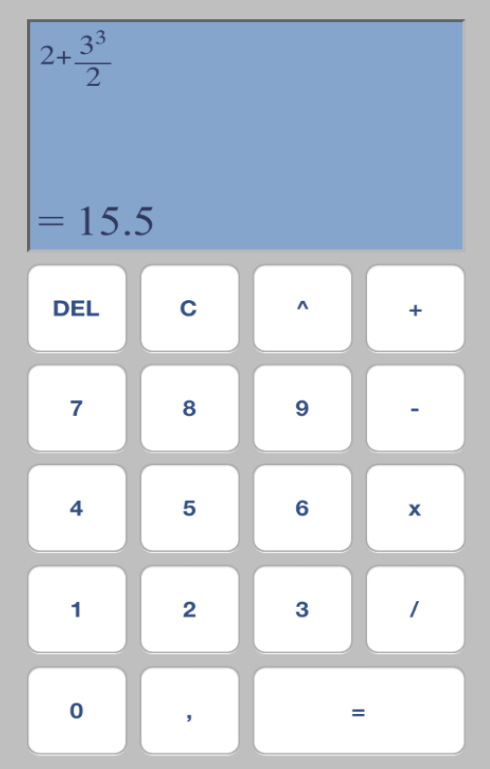
\includegraphics[height=.5\textheight]{portrait.png}
\end{figure}
Die Portrait-View stellt einen einfachen Taschenrechner mit minimalen Grundfunktionen zur Verfügung. Im Display wird oben der eingegebene Ausdruck angezeigt und unten das zurückgegebene Ergebnis.
Zu groß geratene Ausdrücke können mit einem Wischen über das Display gescrollt werden.

\section{Landscape-View}
\begin{figure}[H]
	\centering
	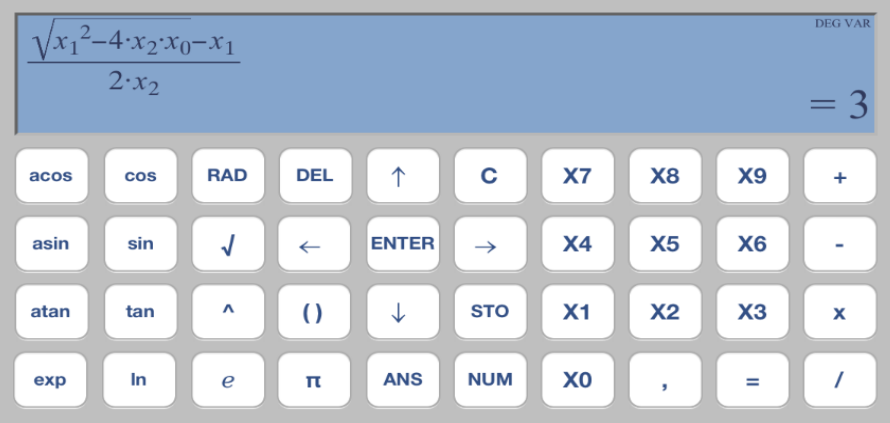
\includegraphics[width=1\textwidth]{landscape.png}
\end{figure}
Dreht man das Gerät in den Landscape Mode, so erhält man den vollen Funktionsumfang des Taschenrechners. 
Im Display erscheint außerdem eine Statusanzeige oben rechts.
\section{Funktionsumfang}
\subsection{Grundlagen}
\subsubsection{Der Platzhalter}
Am Anfang eines leeren Ausdrucks oder nach der Eingabe eines Operators erscheint ein Platzhalter '\_'. 
Dieser fordert dazu auf, eine Zahl, eine Variable, eine Konstante oder eine Funktion einzugeben. Die Operatoren sind dabei gesperrt (Ausnahme: \key{-},\key{/}).

\paragraph{Klammern verwenden:}
Da alle Operatoren und Funktionen nur einen Wert im Platzhalter erwarten, muss in Fällen,
in dem ein neuer Ausdruck benötigt wird, die \key{( )}-Taste gedrückt werden. 
Diese leitet eine neuen Unterausdruck ein.
\paragraph{Hinweis:} Anhand der Ausdrucksausgabe ist nicht immer erkennbar, ob man sich gerade in einem geklammerten Ausdruck befindet. Deshalb wird in diesem Fall in der Statusanzeige '( )' angezeigt. 
\subsubsection{Navigation und der Focus}
Der Focus hebt das aktuelle Element hervor. Mittels \key{$\leftarrow$} und \key{$\rarr$} kann der Focus nach links oder rechts auf dem Ausdruck bewegt werden. 
Ist der Focus am linken oder rechten Ende angekommen wechselt der Focus auf eine Ausdrucksebene höher. 
Die Ausdrucksebenen ergeben sich durch die Eingabe von Klammern und Operatoren wobei Einzelelemente wie Zahlen immer ganz unten stehen. 

Mittels \key{ENTER} kann in einen markierten Ausdruck eingetreten, also auf eine Ebene tiefer gewechselt werden.
\subsubsection{Zahlen}
Über den Nummernblock können Zahlen und ein Komma eingegeben werden.
Neue Ziffern werden an die Zahl angehängt. Beim Drücken eines Operators wird die Zahleneingabe verlassen.
\subsubsection{Operatoren}
Durch Operatoren können Werte von Elementen verknüpft werden. 
Wird ein Operator gedrückt, wenn ein Element im Focus steht, so wird dieses mit einem neuen Platzhalter verknüpft. Dabei spielt die Auswertungsreihenfolge (es gilt Punkt-vor-Strich) eine Rolle:
\begin{enumerate}
	\item Es werden zuerst Ausdrücke in Klammern und Funktionswerte berechnet.
	\item der Exponentenoperator \key{\^{ }}, der eine Zahl hoch einem Exponenten nimmt.
	\item \key{$\times$} und \key{/}
	\item zuletzt \key{+} und \key{-}
\end{enumerate}
\subsubsection{Auswertung}
Drückt man \key{=} so wird der eingegebene Ausdruck ausgerechnet und das Ergebnis am unteren Displayrand angezeigt. 

Bei fehlerhaften Eingaben (z.B. Teilen durch 0) wird 'ERROR' zurückgegeben
\paragraph{Sonderfunktionen:}
\begin{description}
	\item [\key{-}] Wird auf einem Platzhalter Minus gedrückt, so wird dieser bzw. der spätere enthaltene Wert negiert. Erneutes Drücken entfernt das '-'.   
	\item [\key{/}] Wie \key{-}. Allerdings wird der enthaltene Wert invertiert 
		(entspricht $x^{-1} = \frac 1 x$).
\end{description}

\subsection{Weitere Funktionalitäten}
\subsubsection{Mathematische Funktionen}
Drückt man auf eine Funktion so erscheint ein neues Funktionsobjekt im Ausdruck.
Dabei wird ein Platzhalter geschaffen, der die oben beschriebenen Eigenschaften erfüllt.
Bei der Auswertung wird dann der Wert (oder Ausdruck) rechts neben der Funktion in die Funktion eingesetzt und der berechnete Wert zurückgegeben.
\paragraph{Folgende Funktionen sind enthalten:}
\begin{description}
	\item [\key{exp}] Die $e$-Funktion
	\item [\key{$\sqrt{}$}] Die Quadratwurzel
	\item [\key{ln}] Der natürliche Logarithmus
	\item [\key{cos}, \key{sin}, \key{tan}] Die Winkelfunktionen
	\item [\key{acos}, \key{asin}, \key{atan}] Die Umkehrfunktionen der Winkelfunktionen
\end{description}

\subsubsection{Konstanten}
Es ist auch möglich mit symbolischen Konstanten zu rechnen. Deren Werte werden dann beim
Auswerten in die Rechnung eingesetzt
\begin{description}
	\item [\key{$\pi$}] die Kreiszahl $\pi$
	\item [\key{$e$}] die eulersche Zahl
\end{description}

\subsubsection{Variablen}
\paragraph{Variablen}
\begin{figure}[H]
	\centering
	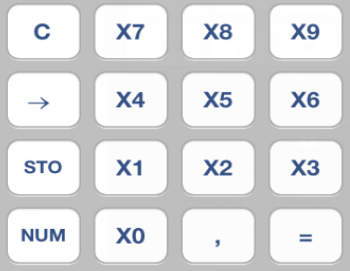
\includegraphics[width=.3\textwidth]{landscape_var.png}
\end{figure}
Drückt man die \key{VAR}-Taste dann wechseln die Ziffern des Nummernblocks auf \key{X0} bis \key{X9}. Die Taste \key{VAR} verändert dabei ihren Titel zu \key{NUM}. In der Statusanzeige wechselt zudem das Symbol 'NUM' auf 'VAR'. Der Rechner befindet sich also im Variablenmodus.

Drückt man nun auf eine der Nummerblocktasten so wird die entsprechende Variable in den Ausdruck eingesetzt.
Beim Berechnen wird dann der Wert aus der Variable entnommen und in den Ausdruck eingefügt.

Durch erneutes Drücken der \key{NUM/VAR}-Taste kann wieder zum Nummernmodus zurückgekehrt werden.
\subparagraph{Hinweis:} Alle Variablen werden mit 0 initialisiert

\paragraph{Speichern}
Beim Betätigen von \key{STO} wechselt der Nummernblock in den Variablenmodus. 
Wird nun eine Variable ausgewählt, wird diese mit einem Zuweisungspfeil links neben den Ausdruck geschrieben.
Nach dem Bestätigen von \key{=} wird der Wert im Ausdruck ermittelt und in der Variable gespeichert.

\paragraph{ANS}
Unabhängig von den oben genannten Variablen wird immer der letzte berechnete Wert in die
ANS-Variable gespeichert. Diese kann man wie eine Variable über die \key{ANS}-Taste in den Ausdruck einsetzen.

\subsubsection{Sondertasten}
\begin{description}
	\item[\key{RAD} / \key{DEG} ]
		Damit lässt sich der Winkelmodus für die Winkelfunktionen von Grad (DEG) auf Bogenmaß (RAD) verändern.
		Der aktuelle Zustand wird in der Statusanzeige ausgegeben.
	\item[\key{DEL}]
		mit dieser Taste lassen sich einzelne Elemente oder ganze Teilausdrücke löschen.
		\begin{itemize}
			\item befindet sich der Focus innerhalb einer Zahl, wird die letzte Ziffer gelöscht.
			\item befindet sich der Focus auf einem Element oder (Teil-) Ausdruck, dann wird der gesamte Teil durch einen Platzhalter ersetzt.
			\item auf einem Platzhalter wird auch der letzte zugehörige Operator (oder die zug. Funktion) gelöscht.
		\end{itemize}
	\item[\key{C}]
		Damit wird der aktuelle Ausdruck zurückgesetzt.
	\item[\key{$\uparrow$}, \key{$\downarrow$}]
		Damit kann über vorher eingegebene Ausdrücke rück- oder vorwärts navigiert werden.
		Mittels \key{ENTER} kann auch in einen ausgewählten Ausdruck wieder eingetreten werden.
\end{description}


